\documentclass[margin=10pt]{standalone}
\usepackage{cmbright}
%\renewcommand{\familydefault}{\sfdefault}
%
\usepackage{tikz}
\usetikzlibrary{arrows}
\usetikzlibrary{arrows.meta}
\usetikzlibrary{backgrounds}
\usetikzlibrary{decorations.markings}
\usetikzlibrary{fit}
\usetikzlibrary{matrix}
\usetikzlibrary{positioning}
\usetikzlibrary{shadows}

\begin{document}
{
\normalsize
%\large

\newsavebox\mybox
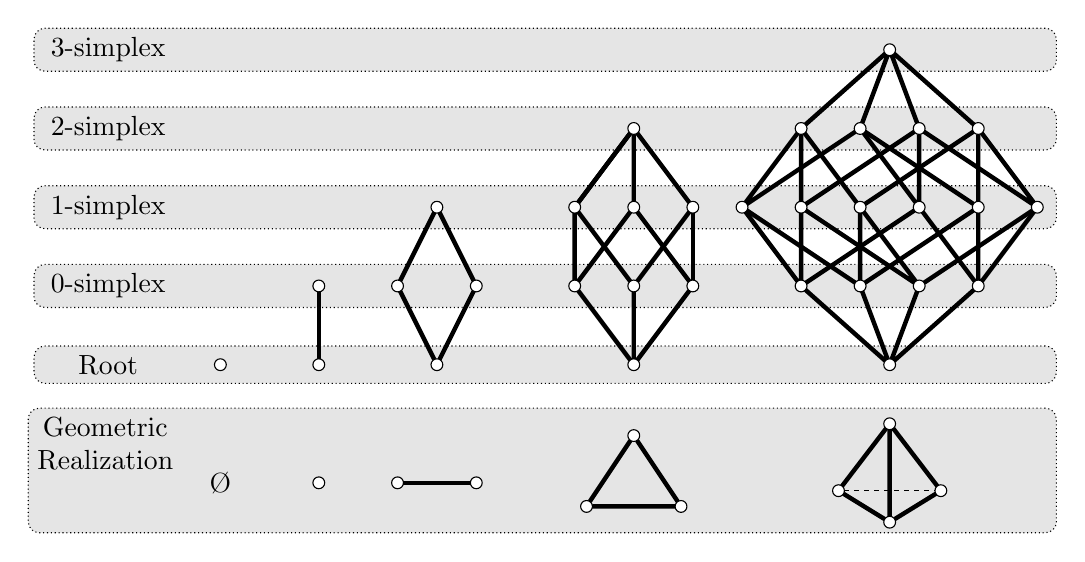
\begin{tikzpicture}[
		every node/.style = {
			draw,
			fill = white!5,
			align = center,
		},
		labeltxt/.style = {
			draw = none,
			fill = none,
			anchor = east,
			minimum width = 1.65cm,
			outer sep = 0,
			inner sep = 0,
		},
		line/.style = {
			ultra thick,
		},
		point/.style = {
			%fill=black,
			inner sep = 0pt,
			outer sep = 0pt,
			minimum size = 1.5mm, 
			circle,
		},
		bgbox/.style = {
			densely dotted,
			rounded corners,
			fill = black!10,
			%drop shadow,
		},
 		]

	%\draw[step=1cm,black!80,very thin] (0,0) grid (15,8);
	%\draw[step=0.5cm,black!20,very thin] (0,0) grid (15,8);

	\pgfmathsetlengthmacro{\base}{1cm};
	\pgfmathsetlengthmacro{\vb}{2cm};
	\pgfmathsetlengthmacro{\offset}{2cm};
	\pgfmathsetlengthmacro{\vo}{1cm};

	\pgfmathsetlengthmacro{\rad}{0.75mm};

	% NULL SET
	\node[point] (0n) at (\base,\vb) {};


	\pgfmathsetlengthmacro{\base}{2.25cm};
	% VERTEX
	\node[point] (1n) at (\base,\vb) {};
	\node[point] (11) at (\base,\vb+\vo) {};
	\draw[line] (1n) -- (11);


	\pgfmathsetlengthmacro{\base}{3.75cm};
	\pgfmathsetlengthmacro{\ho}{0.5cm};
	% EDGE
	\node[point] (2n) at (\base,\vb) {};
	\node[point] (21a) at (\base-\ho,\vb+\vo) {};
	\node[point] (21b) at (\base+\ho,\vb+\vo) {};
	\node[point] (22) at (\base, \vb+2*\vo) {};
	\draw[line] (2n) -- (21a) -- (22) -- (21b) -- (2n);

	
	\pgfmathsetlengthmacro{\base}{6.25cm};
	\pgfmathsetlengthmacro{\ho}{0.75cm};
	% TRIANGLE
	\node[point] (3n) at (\base,\vb) {};
	\node[point] (31a) at (\base,\vb+\vo) {};
	\node[point] (31b) at (\base-\ho,\vb+\vo) {};
	\node[point] (31c) at (\base+\ho,\vb+\vo) {};
	\node[point] (32a) at (\base, \vb+2*\vo) {};
	\node[point] (32b) at (\base-\ho, \vb+2*\vo) {};
	\node[point] (32c) at (\base+\ho, \vb+2*\vo) {};
	\node[point] (33) at (\base, \vb+3*\vo) {};
	\draw[line] (3n) -- (31a) -- (32b) -- (33);
	\draw[line] (31a) -- (32c) -- (33);
	\draw[line] (3n) -- (31b) -- (32b) -- (33);
	\draw[line] (31b) -- (32a);
	\draw[line] (3n) -- (31c) -- (32a) -- (33);
	\draw[line] (31c) -- (32c);

	\pgfmathsetlengthmacro{\base}{9.5cm};
	\pgfmathsetlengthmacro{\ho}{0.75cm};
	% TETRAHEDRON
	\node[point] (4n) at (\base,\vb) {};

	\node[point] (41a) at (\base-1.5*\ho,\vb+\vo) {};
	\node[point] (41b) at (\base-\ho/2,\vb+\vo) {};
	\node[point] (41c) at (\base+\ho/2,\vb+\vo) {};
	\node[point] (41d) at (\base+1.5*\ho,\vb+\vo) {};

	\node[point] (42a) at (\base-2.5*\ho, \vb+2*\vo) {};
	\node[point] (42b) at (\base-1.5*\ho, \vb+2*\vo) {};
	\node[point] (42c) at (\base-\ho/2, \vb+2*\vo) {};
	\node[point] (42d) at (\base+\ho/2,\vb+2*\vo) {};
	\node[point] (42e) at (\base+1.5*\ho,\vb+2*\vo) {};
	\node[point] (42f) at (\base+2.5*\ho,\vb+2*\vo) {};

	\node[point] (43a) at (\base-1.5*\ho,\vb+3*\vo) {};
	\node[point] (43b) at (\base-\ho/2,\vb+3*\vo) {};
	\node[point] (43c) at (\base+\ho/2,\vb+3*\vo) {};
	\node[point] (43d) at (\base+1.5*\ho,\vb+3*\vo) {};

	\node[point] (44) at (\base,\vb+4*\vo) {};
	
	\draw[line] (4n) -- (41a) (4n) -- (41b) (4n) -- (41c) (4n) -- (41d);
	\draw[line] (41a) -- (42a) (41a) -- (42b) (41a) -- (42d);
	\draw[line] (41b) -- (42a) (41b) -- (42c) (41b) -- (42e);
	\draw[line] (41c) -- (42b) (41c) -- (42c) (41c) -- (42f);
	\draw[line] (41d) -- (42d) (41d) -- (42e) (41d) -- (42f);
	\draw[line] (42a) -- (43a) (42a) -- (43b);
	\draw[line] (42b) -- (43a) (42b) -- (43c);
	\draw[line] (42c) -- (43a) (42c) -- (43d);
	\draw[line] (42d) -- (43b) (42d) -- (43c);
	\draw[line] (42e) -- (43b) (42e) -- (43d);
	\draw[line] (42f) -- (43c) (42f) -- (43d);
	\draw[line] (43a) -- (44) (43b) -- (44) (43c) -- (44) (43d) -- (44);

	%% DUMMY POINTS
	\pgfmathsetlengthmacro{\base}{0.4cm};
	\node[labeltxt] (rs) at (\base,\vb) {Root};
	\node[labeltxt] (0s) at (\base,\vb+\vo) {0-simplex};
	\node[labeltxt] (1s) at (\base,\vb+2*\vo) {1-simplex};
	\node[labeltxt] (2s) at (\base,\vb+3*\vo) {2-simplex};
	\node[labeltxt] (3s) at (\base,\vb+4*\vo) {3-simplex};

	\pgfmathsetlengthmacro{\base}{11.5cm};
	\node[labeltxt] (rd) at (\base,\vb) {};
	\node[labeltxt] (0d) at (\base,\vb+\vo) {};
	\node[labeltxt] (1d) at (\base,\vb+2*\vo) {};
	\node[labeltxt] (2d) at (\base,\vb+3*\vo) {};
	\node[labeltxt] (3d) at (\base,\vb+4*\vo) {};

	\begin{scope}[on background layer]
		\node[bgbox,
		      fit=(rs)(rd)
		     ]
		    (root){};
	\end{scope}
	\begin{scope}[on background layer]
		\node[bgbox,
		      fit=(0s)(0d)
		     ]
		    (0simp){};
	\end{scope}
	\begin{scope}[on background layer]
		\node[bgbox,
		      fit=(1s)(1d)
		     ]
		    (1simp){};
	\end{scope}
	\begin{scope}[on background layer]
		\node[bgbox,
		      fit=(2s)(2d)
		     ]
		    (2simp){};
	\end{scope}
	\begin{scope}[on background layer]
		\node[bgbox,
		      fit=(3s)(3d)
		     ]
		    (3simp){};
	\end{scope}

	%% CORRESPONDING SHAPES
	\pgfmathsetlengthmacro{\vb}{0cm};
	\node[draw = none, fill= none] (ns) at (1cm,\vb+0.5*\vo) {\O};	

	\pgfmathsetlengthmacro{\base}{2.25cm};
	\node[point] (vertex) at (\base,\vb+0.5*\vo) {};	
	
	\pgfmathsetlengthmacro{\base}{3.75cm};
	\pgfmathsetlengthmacro{\ho}{0.5cm};
	\node[point] (e1) at (\base-\ho,\vb+0.5*\vo) {};
	\node[point] (e2) at (\base+\ho,\vb+0.5*\vo) {};
	\draw[line] (e1) -- (e2);

	\pgfmathsetlengthmacro{\base}{6.25cm};
	\pgfmathsetlengthmacro{\ho}{0.6cm};
	\node[point] (t1) at (\base-\ho,\vb+2mm) {};
	\node[point] (t2) at (\base+\ho,\vb+2mm) {};
	\node[point] (t3) at (\base, \vb+1.1*\vo) {};
	\draw[line] (t1) -- (t2) -- (t3) -- (t1);

	\pgfmathsetlengthmacro{\base}{9.5cm};
	\pgfmathsetlengthmacro{\ho}{0.65cm};
	\node[point] (tt1) at (\base,\vb) {};
	\node[point] (tt2) at (\base+\ho,\vb+4mm) {};
	\node[point] (tt3) at (\base, \vb+1.25*\vo) {};
	\node[point] (tt4) at (\base-\ho, \vb+4mm) {};

	\draw[line] (tt1) -- (tt2) -- (tt3) -- (tt1);
	\draw[line] (tt1) -- (tt4) -- (tt3);
	\draw[line, dotted, thin] (tt4) -- (tt2);



	\node[labeltxt] (gr) at (0.4cm,1cm) {Geometric\\Realization};
	\node[labeltxt] (grd) at (11.5cm,0cm) {};
	\begin{scope}[on background layer]
		\node[bgbox,
		      fit=(gr)(grd)
		     ]
		    (grbox){};
	\end{scope}


\end{tikzpicture}
}% end size


\end{document}   